% chapter3 模型

\chapter{基于Inception和混合注意力的运动想象脑电图分类网络构建}

论文前两个章节主要对运动想象脑电图分类领域的基础知识以及相关研究做了一定的介绍,并且对该领域仍然存在的问题进行了分析。本章对这些问题进行进一步的探讨,针对这些问题构建了一种端到端的新模型:首先,以ShallowConvNet为基础,引入深度可分离卷积和轻量级注意力模块,减少网络参数,提高对重要通道数据的关注,同时促进时空特征的深度融合;其次,在以上模型的基础上,引入Inception模块替代时间卷积层,并行提取多尺度的时间特征,对该结构进行进一步改造,将密集连接引入Inception模块的分支中,更好地关注EEG信号的局部细节和浅层特征;最后,引入Transformer模块以更好地利用EEG信号的全局信息,并且针对EEG信号信噪比低的特点,引入软阈值模块对Transformer进行改进,从而减少噪声的干扰。经过以上一系列改进,最终构建了一种基于Inception和混合注意力的运动想象脑电图分类网络HIT-Net,在运动想象脑电图分类任务上能够取得更好的效果。

\section{基于EEGNet和注意力机制的紧凑型基础网络VSNet}

原始的EEG信号通常为二维数据,包括通道(电极)和时间两个维度,具体而言,在EEG信号矩阵中,行代表分布在头皮不同位置的采样通道,列为时间序列数据,每个采样点对应一个时间戳下的生物电信号(通常为电压值),因此,一列数据就是一个特定时间点下所有通道同步采集到的电压读数。原始的EEG信号经过预处理之后,可以转换为时频图、头皮点位拓扑图等输入模式,尽管经过转换的输入相较于原始输入能够更全面地体现EEG信号的时频空信息,但这一过程往往需要具有神经科学背景的人工参与,在增加了人工成本同时,限制了模型自适应学习EEG信号中蕴含的复杂时空特征的能力,此外,复杂的预处理环节也增加了计算开销和应用成本,难以满足BCI系统即时响应的需求。因此,端到端网络在MI-EEG分类领域受到越来越多的重视,这类网络不经过或者仅仅经过很少的预处理步骤,而由深度学习算法自适应地提取关键特征并作出预测。

ShallowConvNet\cite{schirrmeister2017deep}是一个专为端到端解码脑电图(EEG)信号而设计的深度学习架构,其构思源自EEG信号解码研究领域中广泛使用的经典特征提取方法——滤波器组共空间模式(Filter Bank Common Spatial Pattern, FBCSP)\cite{ang2008filter}。ShallowConvNet具有FBCSP算法对频带功率特征高效提取的特性,在实验中证明了能够学习频带功率变化的时间结构特性\cite{schirrmeister2017deep},研究发现,该特性有助于提高分类性能\cite{sakhavi2015parallel}。实验证明,ShallowConvNet在MI-EEG分类领域具有优良的性能\cite{lawhern2018eegnet},同时具有较少的参数量,因此论文以ShallowConvNet为基础搭建紧凑型MI-EEG分类网络。

ShallowConvNet的结构如图~\ref{fig:ShallowConvNet}~所示。ShallowConvNet采用四步流程对原始二维输入数据进行处理。具体而言,ShallowConvNet首先通过时间卷积层捕获信号的时间域特征,再通过空间卷积层捕获这些时间特征在不同通道间的空间关联性,随后通过平均池化层进行下采样,最后通过全连接层将多维特征映射至分类输出空间。ShallowConvNet采取的时间卷积和空间卷积相分离的策略有效地减少了模型参数量,同时,空间卷积核能够学习其对应的时间卷积核提取的特征,这种设计隐含了对FBCSP算法核心思想的借鉴与实现。
\begin{figure}
    \centering
    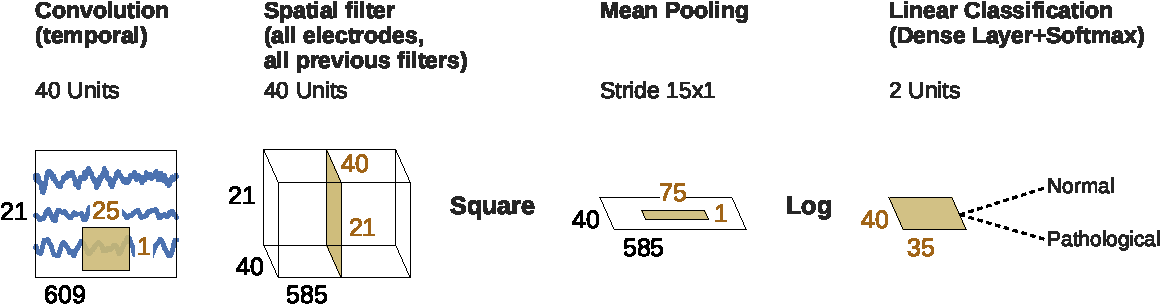
\includegraphics[width=\textwidth]{ShallowNet.pdf}
    \caption{ShallowConvNet结构}
    \label{fig:ShallowConvNet}
\end{figure}

\subsection{注意力机制}

注意力机制的提出受到人类认知科学的启发,其核心理念在于模拟人类大脑在处理信息过程中的选择性关注机制,即并非均匀地分配注意力处理对待所有输入,而是将注意力主动、动态且有选择性地聚焦于最重要或最相关的信息上。自二十世纪被提出以来\cite{730558},注意力机制在计算机视觉、自然语言处理等领域得到了广泛的应用,并表现出了优秀的效果。根据神经科学先验知识,EEG信号中不同的通道和采样点具有不同的重要性,这为在MI-EEG分类领域应用注意力机制提供了理论依据,此外,将二维EEG信号视为一种由通道和时间两个维度构成的特殊图像,使得在MI-EEG分类领域能够迁移应用计算机视觉领域中的注意力机制。

计算机视觉领域中经常使用的注意力机制有:

(1) 通道注意力机制
    
不同于EEG信号中代表电极的通道,计算机视觉领域的通道代表图像的不同特征映射。通道注意力机制用于调整不同特征通道的重要性,通常会对每一个特征通道计算一些全局统计量,如均值、方差等,再将这些统计量经过非线性变换层进行编码,最后将编码向量进行转换并用于各个特征通道的加权。通道注意力机制的经典模型是压缩和激励网络(Squeeze-and-Excitation Networks,SENet)\cite{8578843},其主要思想即是压缩(Squeeze)和激励(Excitation),SENet首先通过压缩操作获取全局上下文信息,然后通过激励操作对每个通道独立生成权重系数。具体而言,在压缩操作中,SENet在空间维度执行全局池化操作,将每个通道的特征图汇总成一个标量值;然后,在激励操作中,SENet通过一个全连接网络生成每个通道的权重系数,这些权重系数用于重新加权每个通道的特征图,以增强有用的特征并抑制无用的特征。

在后文中,为避免与计算机视觉领域中的概念相混淆,在MI-EEG分类任务中,用深度来代表EEG信号的不同特征映射,而通道仍然代表电极。

2. 空间注意力机制
    
在计算机视觉领域中,空间注意力机制用于调整图片、视频等输入数据在空间维度中不同区域的重要性,通常会在深度维度上通过全局池化、卷积、特征融合等操作生成一个与特征图尺寸相同的注意力图,其值反映了空间维度中不同区域的注意力强度,最后,将注意力图进行转换,并用于原始特征图的加权。空间注意力机制的经典模型是空间变换网络(Spatial Transformer Network,STN)\cite{jaderberg2015spatial},其具有对输入数据进行空间变换的能力,能够自动捕获重要区域的特征。

3. 混合注意力机制
    
混合注意力机制是一种集成多种注意力机制(如空间注意力、通道注意力及自注意力等)的方法,旨在更全面地捕获和整合输入数据在不同维度的有效信息。混合注意力机制通常会使用不同的注意力机制分别计算原始特征图的注意力权重,再将这些注意力权重进行融合,最后将融合后的注意力权重用于原始特征图的加权,或者将不同的注意力权重用于原始特征图加权,再将加权特征图进行融合。混合注意力机制的经典模型有卷积注意力机制模块(Convolutional Block Attention Module,CBAM)\cite{woo2018cbam}、空间与通道压缩与激励模块(Spatial and Channel Squeeze-and-Excitation,scSE)\cite{roy2018concurrent}等。
    
CBAM结合了通道注意力机制与空间注意力机制,其结构如图~\ref{fig:CBAM}~所示,输入特征图首先经过通道注意力模块进行加权,再通过空间注意力模块进行加权,从而得到最终结果。
\begin{figure}
    \centering
    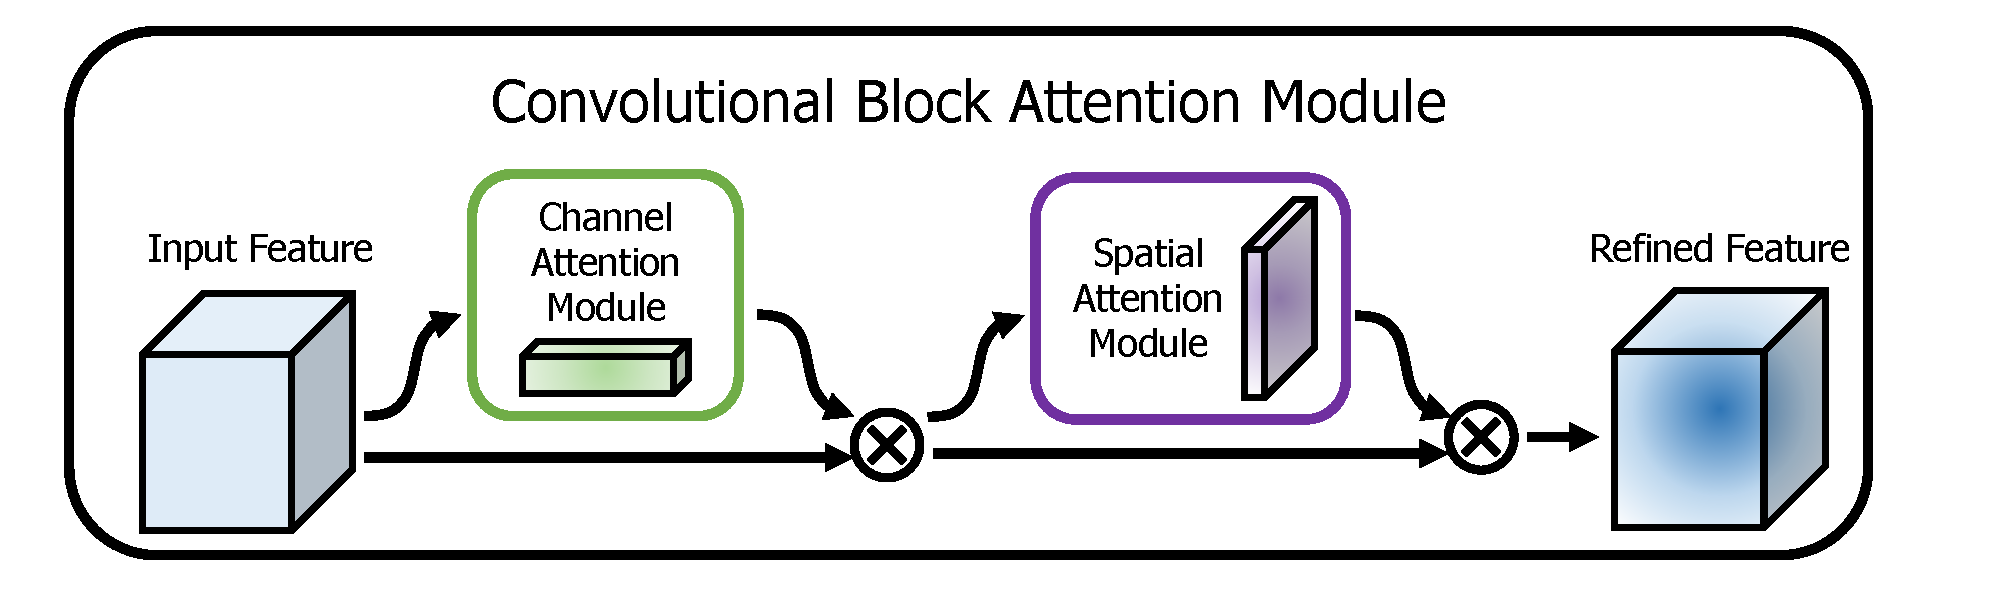
\includegraphics[width=\textwidth]{CBAM.pdf}
    \caption{CBAM结构}
    \label{fig:CBAM}
\end{figure}

具体而言,在通道注意力模块中,输入特征图分别进行空间维度上的全局最大池化和全局平均池化,再将得到的统计值分别通过一个共享权重的全连接层,最后经过逐点加和与非线性变换得到通道注意力权重,用于输入特征图的加权。空间注意力模块的输入是经过通道注意力加权的特征图,首先在通道维度上进行全局最大池化和平均池化,再将得到的统计值在通道维度进行拼接,最后经过卷积降维与非线性变换得到空间注意力权重,与特征图加权后得到最终结果。CBAM的模块结构如图~\ref{fig:CBAM-Block}~所示。
% \begin{figure}[h]
%     \centering
%     \begin{subfigure}{0.45\textwidth}
%       
\includegraphics[width=\linewidth]{whulogo.pdf}
%       \caption{CBAM通道注意力模块结构}
%       \label{fig:CBAM-Channel}
%     \end{subfigure}\qquad
%     \begin{subfigure}{0.45\textwidth}
%       
\includegraphics[width=\linewidth]{whulogo.pdf}
%       \caption{CBAM空间注意力模块结构}
%       \label{fig:CBAM-Spatial}
%     \end{subfigure}
%     \caption{CBAM模块结构}
%     \label{fig:CBAM-Block}
% \end{figure}
\begin{figure}
  \centering
  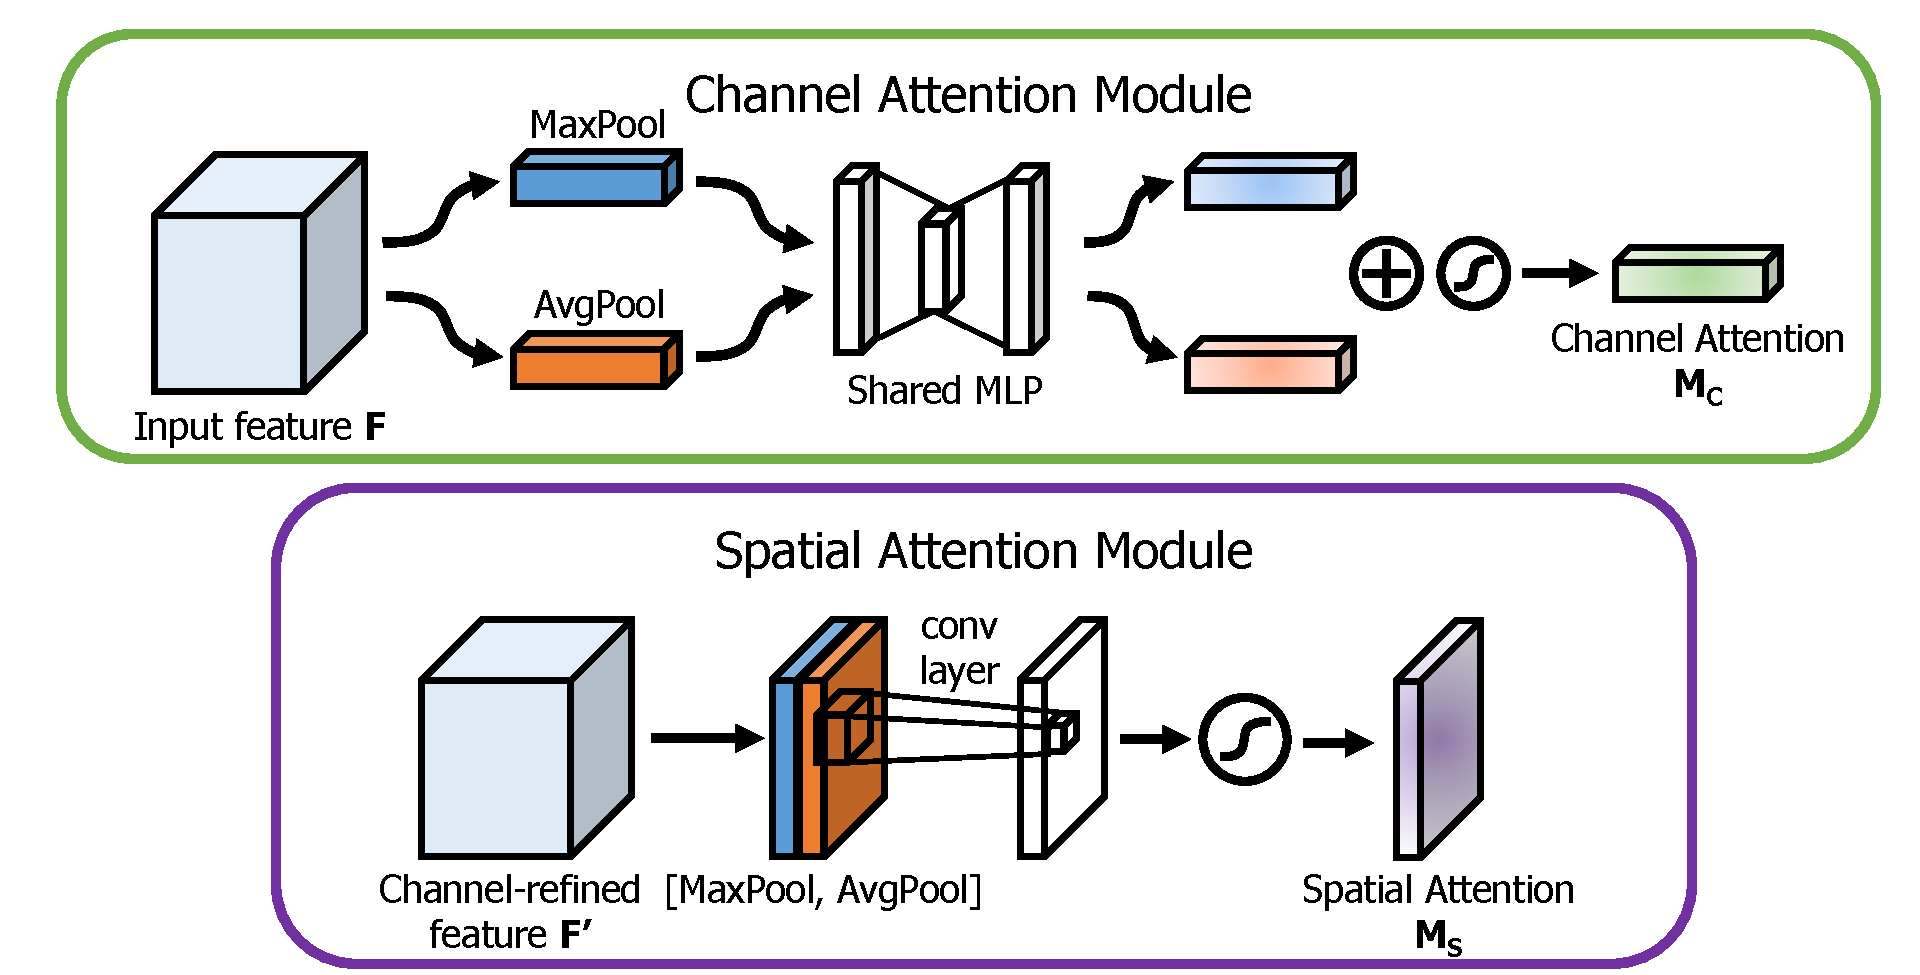
\includegraphics[width=\textwidth]{CBAM-Block.pdf}
  \caption{CBAM模块结构}
  \label{fig:CBAM-Block}
\end{figure}

scSE同样结合了通道注意力机制与空间注意力机制,基于SENet提出了一种通道注意力模块(Channel Squeeze-and-Excitation,cSE)和一种空间注意力模块(Spatial Squeeze-and-Excitation,sSE),其结构如图~\ref{fig:scSE}~所示,不同于CBAM,scSE的两个子模块并行处理原始输入,分别在空间维度和通道维度对原始输入进行加权,最后再进行特征图的融合。具体而言,cSE模块中,原始输入依次经过了空间维度的全局平均池化,通道维度的卷积降维与升维,以及非线性变换,以得到通道注意力权重。sSE模块中,直接通过深度卷积在通道维度进行降维,再经过非线性变换以得到空间注意力权重。
\begin{figure}
    \centering
    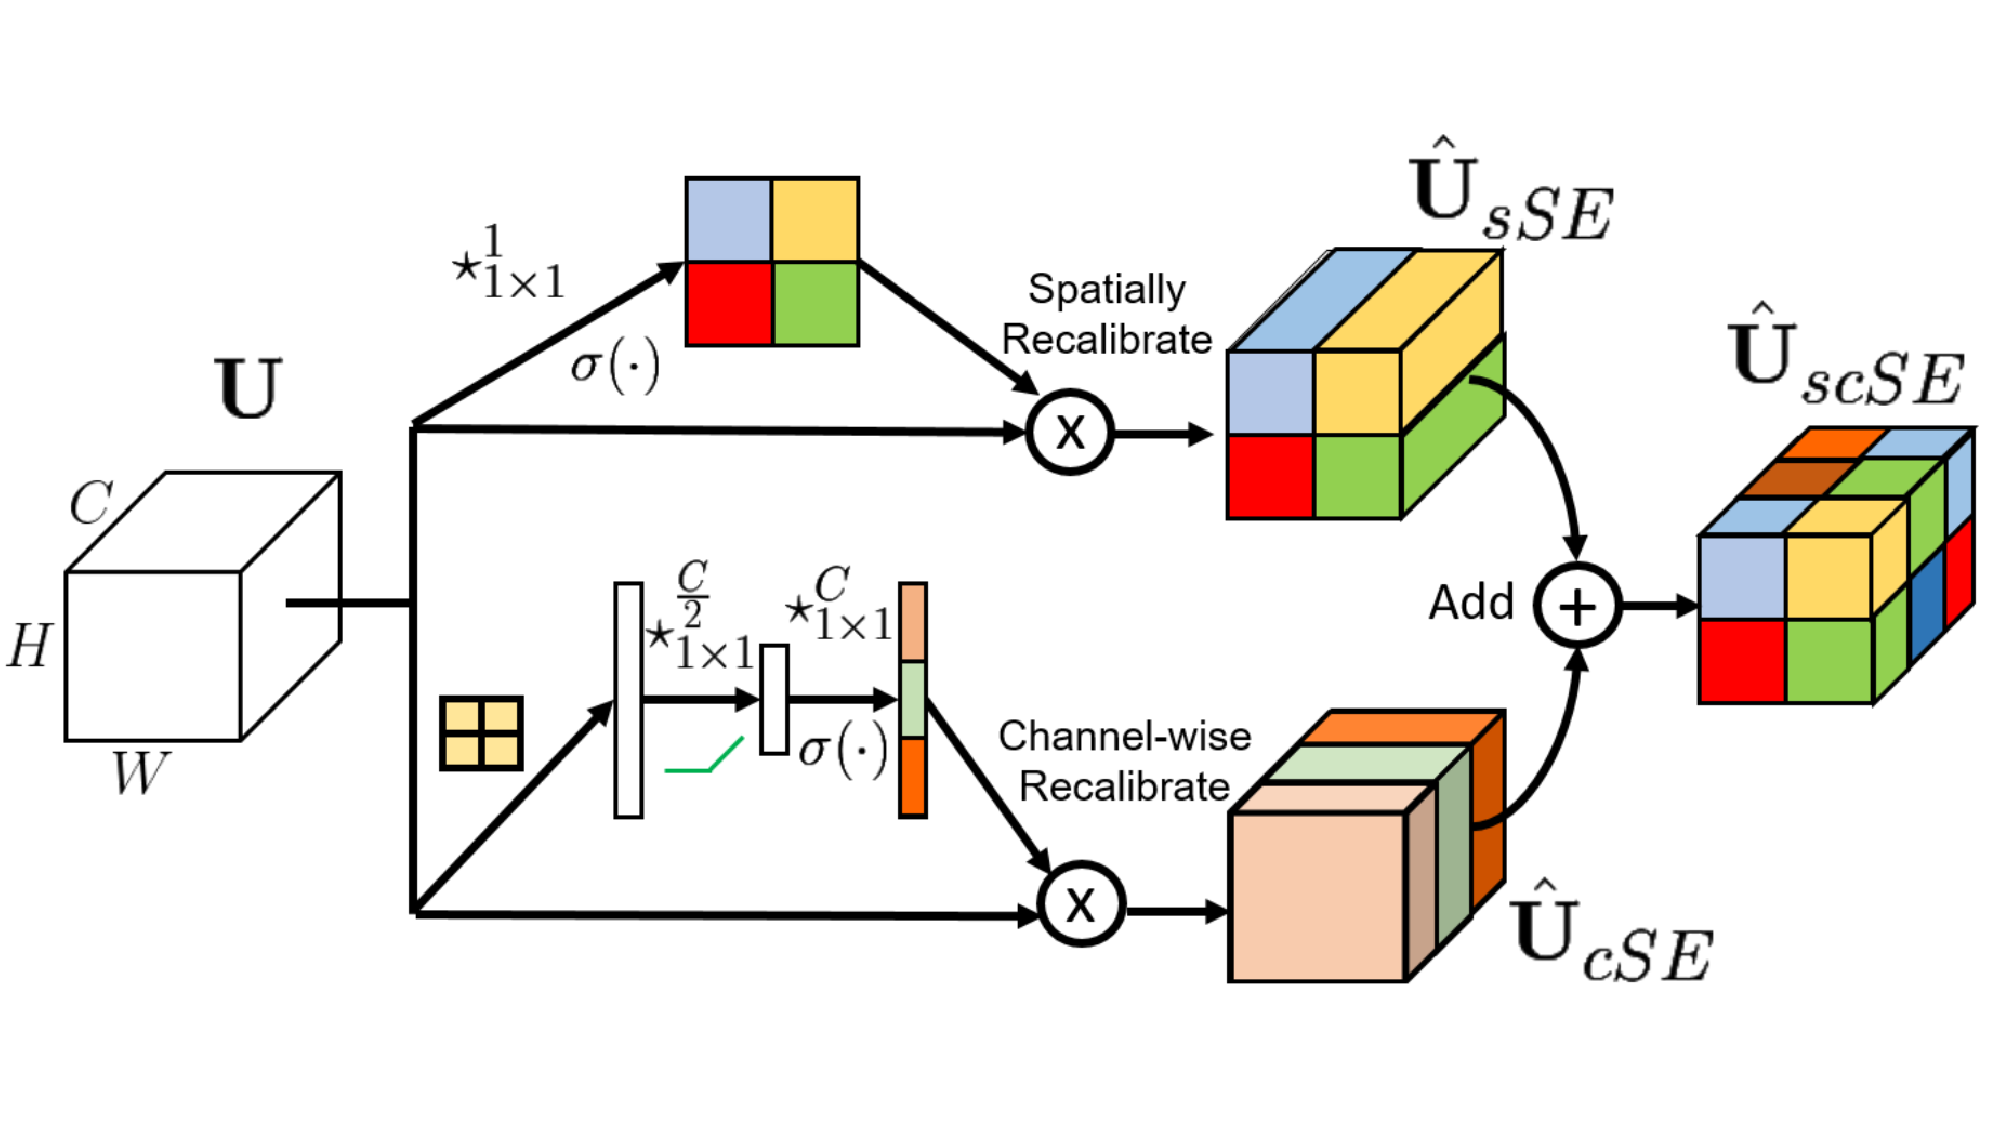
\includegraphics[width=\textwidth]{scSE.pdf}
    \caption{scSE结构}
    \label{fig:scSE}
\end{figure}

\subsection{ShallowConvNet结合注意力机制的紧凑型MI-EEG分类网络}

在上一节中,论文介绍了计算机视觉领域常用的注意力机制,然而,不同于图像数据,EEG信号作为二维输入数据,并不具备深度维度信息,因此,无法直接将计算机视觉领域的注意力机制应用于MI-EEG分类任务中。

文献\cite{lawhern2018eegnet}\cite{schirrmeister2017deep}指出,在EEG信号解码任务中,增加神经网络的深度有利于提升解码精度。瓶颈层(Bottleneck Layer)是深度神经网络中的常见结构\cite{he2016deep}\cite{huang2017densely},通常用于对数据的降维和升维,由于采用了1\times1卷积进行操作,瓶颈层能够有效地减少神经网络的参数。因此,论文将瓶颈层引入ShallowConvNet中,旨在增加较少参数量的情况下对原始输入数据进行升维操作,并在深度维度上促进时空信息的融合。

为了加快网络训练速度,并避免小数据集下过早的过拟合,论文在引入瓶颈层的基础上,对ShallowConvNet的结构进行了进一步的调整:

1. 借鉴EEGNet\cite{lawhern2018eegnet}的结构,将ShallowConvNet的时间卷积和空间卷积替换为参数量更少的深度可分离卷积\cite{lawhern2018eegnet};

2. 由神经科学先验知识可知,通道维度蕴含的信息量通常低于时间维度,因此,在时间卷积层之后使用瓶颈层进行适度的降维,以进一步缩减模型参数;

3. 在模型中引入了一系列正则化技术,包括批量归一化(Batch Normalization,BN)和随机Dropout等。

此外,论文将ShallowConvNet中的对数激活函数替换为GELU激活函数,前者基于FBCSP算法中的对数方差计算提出,后者基于高斯分布和自然梯度流提出,能够更自然地模拟神经元的概率行为,具有更好的连续性和光滑性\cite{hendrycks2016gaussian},实验证明了GELU激活函数较之对数激活函数具有更好的效果。论文将改进后的模型称为Base-ConvNet,并在此基础上引入注意力机制进行进一步优化。

注意力机制通过动态分配权重,使得模型能够聚焦于输入数据中的关键信息,削弱噪声的影响,混合注意力机制则结合了多种注意力机制的优点,从而能够更全面地捕获和整合不同维度的数据特征,并在许多情况下展现出优于单一注意力机制的性能。因此,论文将升维处理后的EEG信号视作具有深度信息的图像数据,采用结合了深度注意力和空间注意力的混合注意力机制对Base-ConvNet进行改进。

CBAM模块和scSE模块均为轻量级注意力模块,且均兼顾深度注意力和空间注意力,但scSE模块在参数数量上更具优势。与此同时,文献\cite{roy2018concurrent}研究发现scSE模块在语义分割任务上表现出色,特别是在与EEG信号拥有相似生理特性的医学图像的分割任务,其性能优于CBAM模块。基于以上理由,论文选择将scSE模块引入Base-ConvNet模型中,构建紧凑型MI-EEG分类网络。由于Base-ConvNet的特征提取过程分为时间卷积和空间卷积两个阶段,scSE模块可采取以下三种引入方式:其一是在时间卷积层后引入;其二是在空间卷积层后引入;其三是同时在时间卷积层和空间卷积层之后引入。图~\ref{fig:att-Base}~展示了这三种引入scSE模块的方式,从左至右分别是时间卷积层后引入scSE模块、空间卷积层后引入scSE模块,以及在时间卷积和空间卷积层后均引入scSE模块。将这三种引入方式对应的模型分别简称为S-Temporal-BaseNet、S-Spatial-BaseNet、S-TS-BaseNet。
\begin{figure}
  \centering
  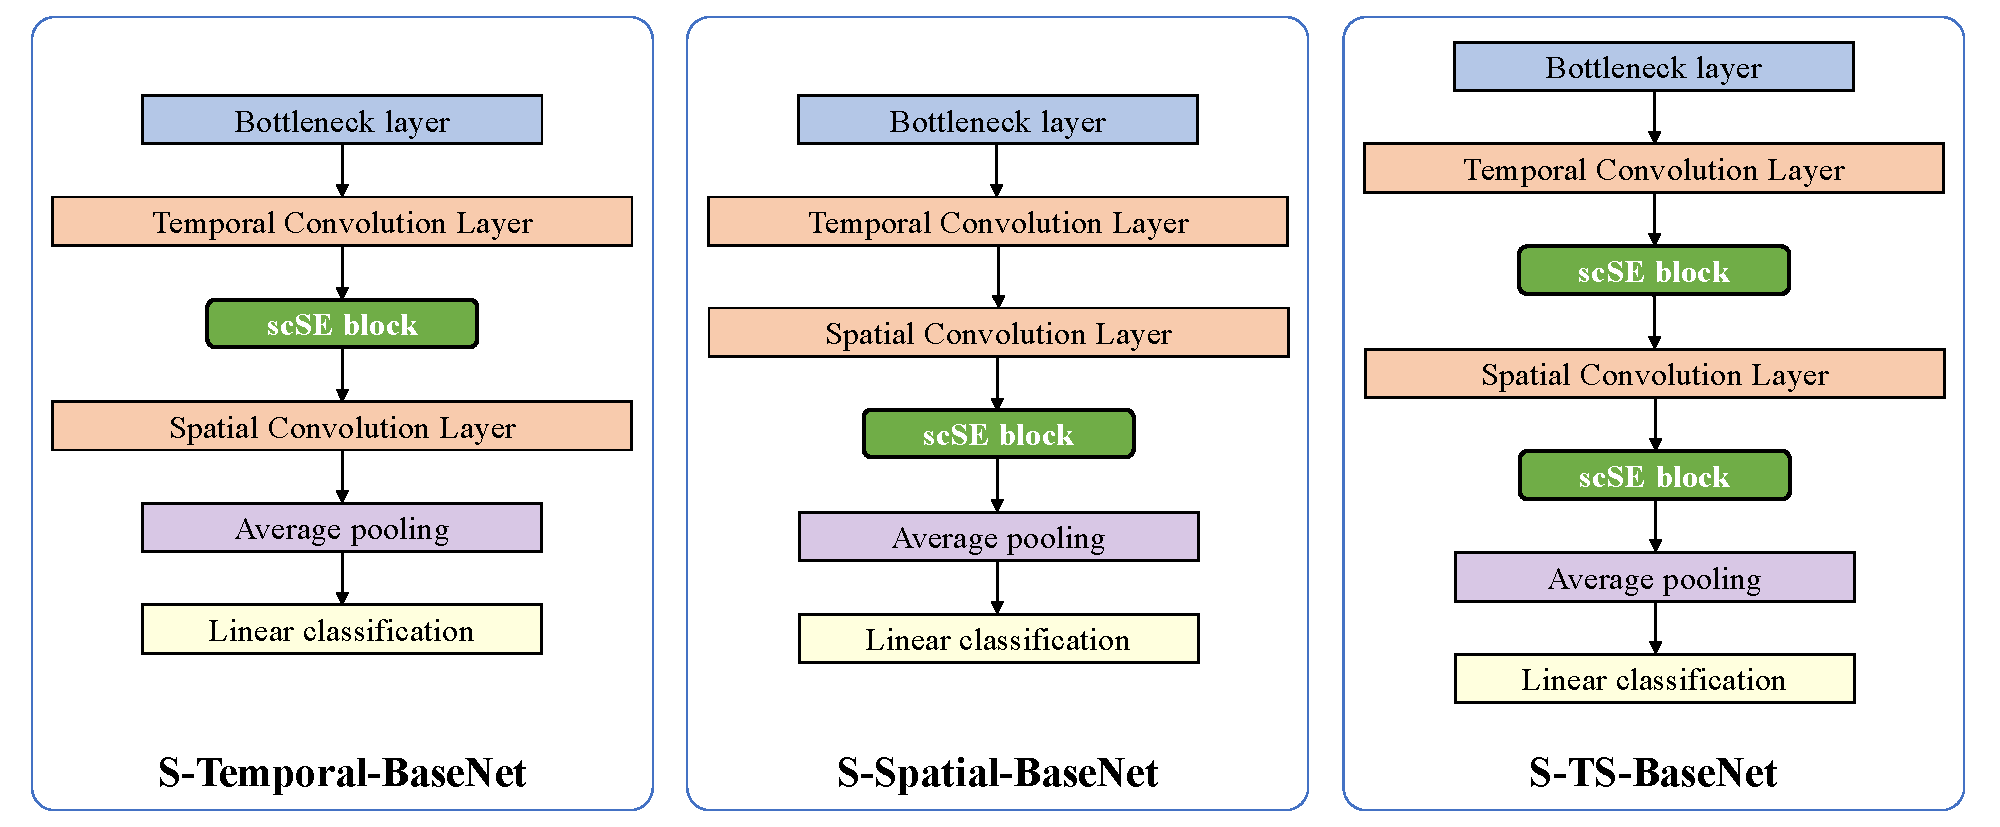
\includegraphics[width=\textwidth]{att-Base.pdf}
  \caption{Base-ConvNet引入注意力模块的方式}
  \label{fig:att-Base}
\end{figure}

表~\ref{tab:scSE-BaseNet}~展示了S-Temporal-BaseNet、S-Spatial-BaseNet、S-TS-BaseNet三种模型在BCI Competition IV Dataset 2A\cite{tangermann2012review}数据集上的对比实验结果。实验采用固定的参数,表格中展示的准确率(Accuracy,ACC)和Kappa一致性系数(Kappa)指标为数据集中九位受试者的平均表现,标准差(Standard Deviation,SD)则为准确率的标准差。从准确率和一致性分析,S-ST-BaseNet模型的效果优于其他两种模型,与经验相符。此外,S-Temporal-BaseNet模型的效果优于S-Spatial-BaseNet模型,其原因可能在于,空间卷积层沿通道维度的卷积和沿深度维度的降维使得数据损失了部分特征,进而减弱了scSE模块提取关键特征权重的能力,而时间卷积层保留了大部分深度信息和通道信息,因此,在时间卷积层之后加入scSE模块能够帮助模型更好地捕捉深度和空间的特征。从标准差分析,S-TS-BaseNet模型的准确率波动幅度较小,对不同受试者的MI-EEG分类效果相对均衡,另外两种模型在不同受试者间的分类精度则存在较为明显的差异。实验数据显示,S-TS-BaseNet模型在增加了少量参数的情况下,取得了更好的效果,因此,论文采用同时在时间卷积层和空间卷积层之后引入scSE模块的方式,构建基于ShallowConvNet和scSE模块的紧凑型MI-EEG分类网络,后文称为S-BaseNet。
\begin{table}[ht]
  \centering
  \caption{scSE模块引入位置对比}
  \label{tab:scSE-BaseNet}
  \begin{tabularx}{\textwidth}{CCCCC}
    \toprule
    \makebox[0.2\textwidth][c]{Models} & \makebox[0.2\textwidth][c]{ACC(\%)} & \makebox[0.2\textwidth][c]{Kappa} & \makebox[0.2\textwidth][c]{SD} & \makebox[0.2\textwidth][c]{Parameters} \\
    % Models & ACC(\%) & Kappa & SD & Parameters \\
    \midrule
    \makebox[0.2\textwidth][c]{S-Temporal-BaseNet} & \makebox[0.2\textwidth][c]{78.09} & \makebox[0.2\textwidth][c]{0.71} & \makebox[0.2\textwidth][c]{10.38} & \makebox[0.2\textwidth][c]{4702} \\
    \makebox[0.2\textwidth][c]{S-Spatial-BaseNet} & \makebox[0.2\textwidth][c]{77.16} & \makebox[0.2\textwidth][c]{0.69} & \makebox[0.2\textwidth][c]{10.24} & \makebox[0.2\textwidth][c]{\textbf{4357}} \\
    \makebox[0.2\textwidth][c]{S-TS-BaseNet} & \makebox[0.2\textwidth][c]{\textbf{78.55}} & \makebox[0.2\textwidth][c]{\textbf{0.71}} & \makebox[0.2\textwidth][c]{\textbf{9.46}} & \makebox[0.2\textwidth][c]{4765} \\
    \bottomrule
  \end{tabularx}
\end{table}


S-BaseNet的结构如图~\ref{fig:S-BaseNet}~所示。在ShallowConvNet的基础上,引入了瓶颈层用于数据的升维和降维,同时,将时间卷积和空间卷积替换为深度可分离卷积,并在时间卷积层和空间卷积层之后增加了scSE注意力模块,其通过深度注意力机制和空间注意力机制对特征图进行注意力加权,从而增强模型对于关键特征的关注度。相较于传统卷积神经网络,S-BaseNet具有较小的参数规模,在减小计算开销的同时能够缓解过拟合现象。
\begin{figure}
  \centering
  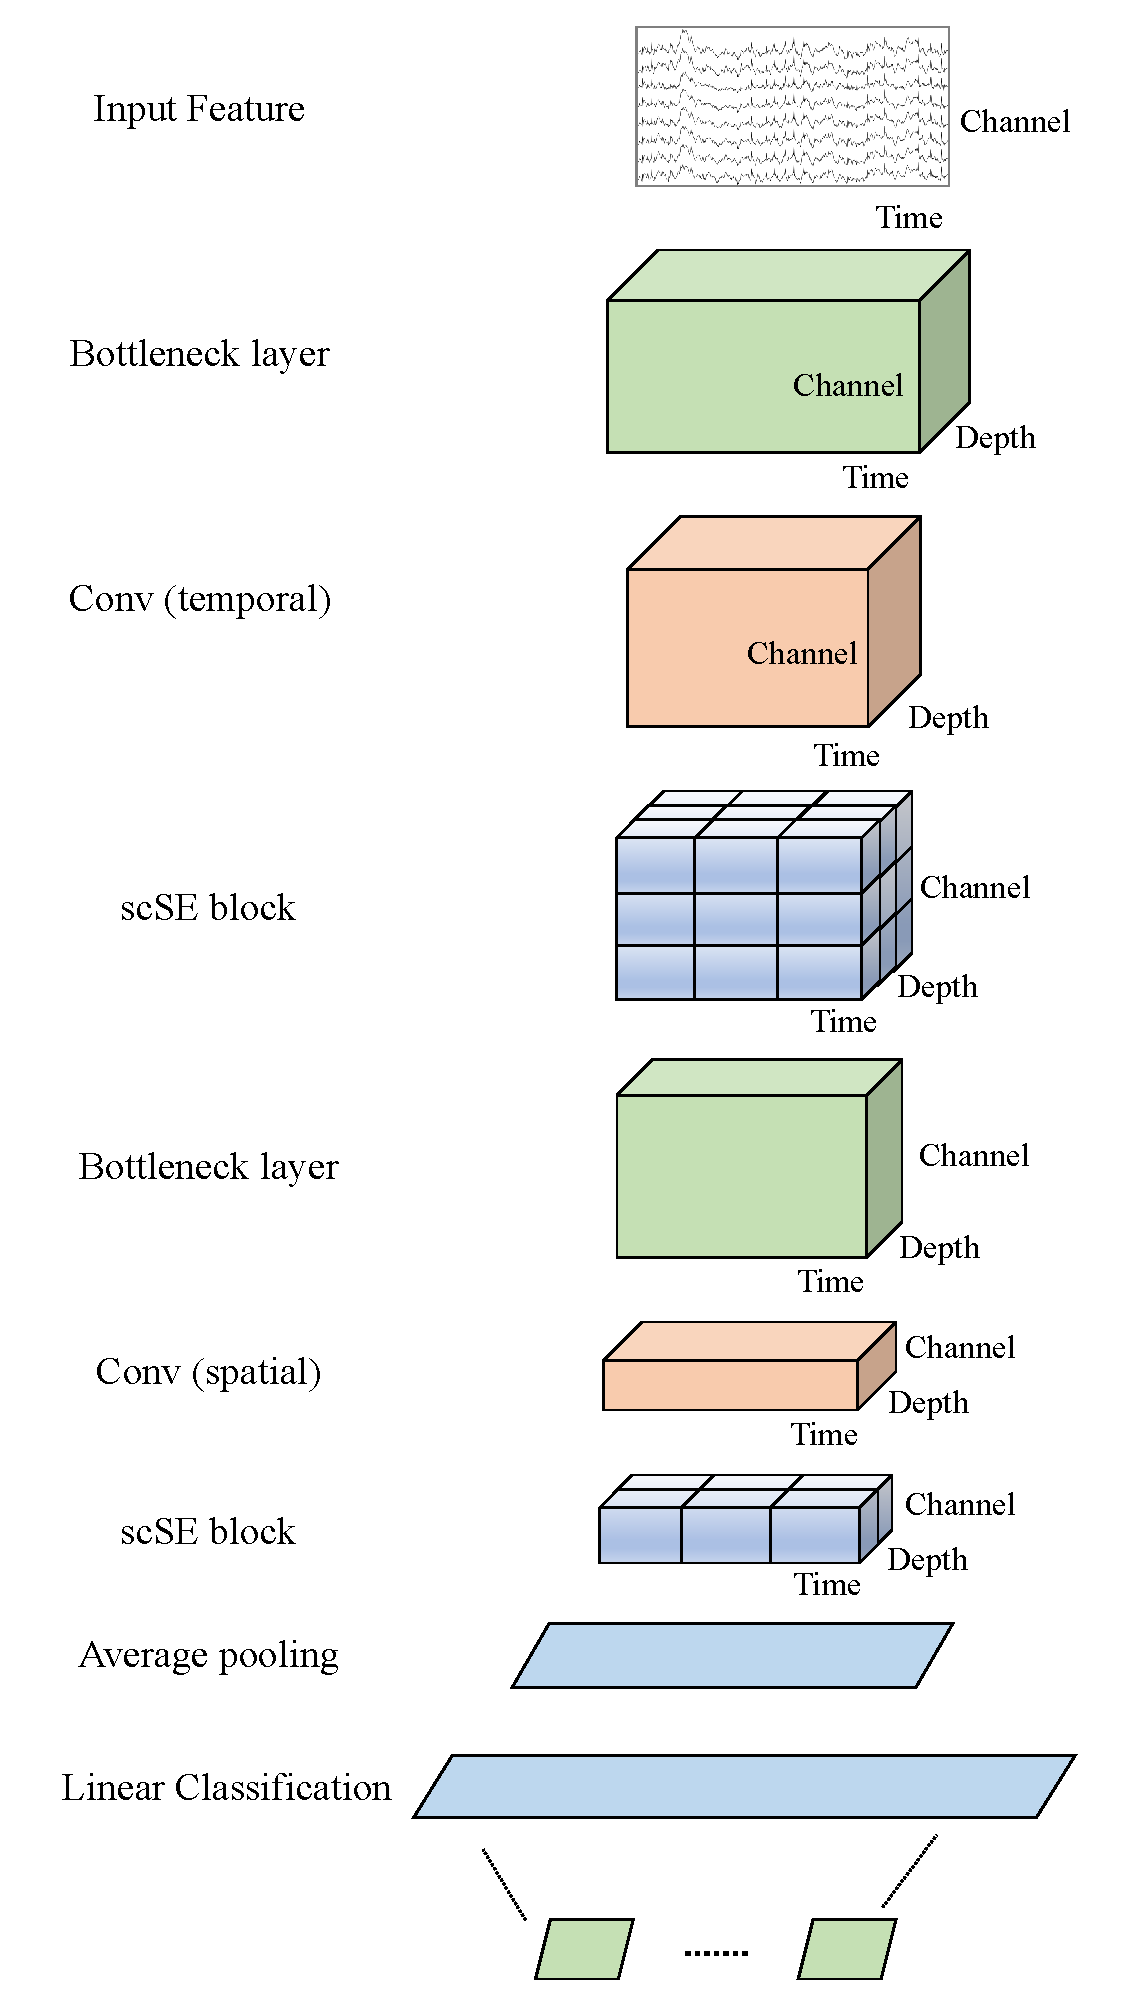
\includegraphics[height=0.8\textwidth]{S-BaseNet.pdf}
  \caption{S-BaseNet结构}
  \label{fig:S-BaseNet}
\end{figure}

为进一步提升S-BaseNet模型性能,对其中的scSE模块进行改进。针对sSE模块,论文从CBAM模块的多维全局池化思想以及FBCNet模型的方差层设计\cite{mane2021fbcnet}得到启发,采用深度维度上的全局平均池化和全局方差计算操作代替原模块中的压缩操作,随后通过深度卷积对深度维度的特征图进行聚合,在更好地表征EEG信号特性的同时,进一步降低了参数规模。针对cSE模块,采用全局最大池化取代全局平均池化操作,实验证明了这一改动使模型具有更好的效果。此外,将scSE模块中的Sigmoid激活函数替换为Softmax激活函数,旨在更好地利用全局信息。论文将改良后的scSE模块称为V-scSE(Variance-Informed Spatial and Channel Squeeze-and-Excitation)模块,其结构如图~\ref{fig:V-scSE}~所示。使用V-scSE模块替换S-BaseNet模型中的scSE模块,最终得到ShallowConvNet结合V-scSE混合注意力模块的紧凑型端到端MI-EEG分类网络VSNet。VSNet网络结构能够直接处理未经过复杂预处理的原始EEG信号,其较小的参数规模不仅有助于缓解过拟合现象,还有利于降低计算资源消耗,提升训练速度。与此同时,ShallowConvNet结合V-scSE模块的架构增强了网络对EEG信号重要特征的关注度,实现了MI-EEG分类精度的提升,取得了较为理想的性能表现。
\begin{figure}
  \centering
  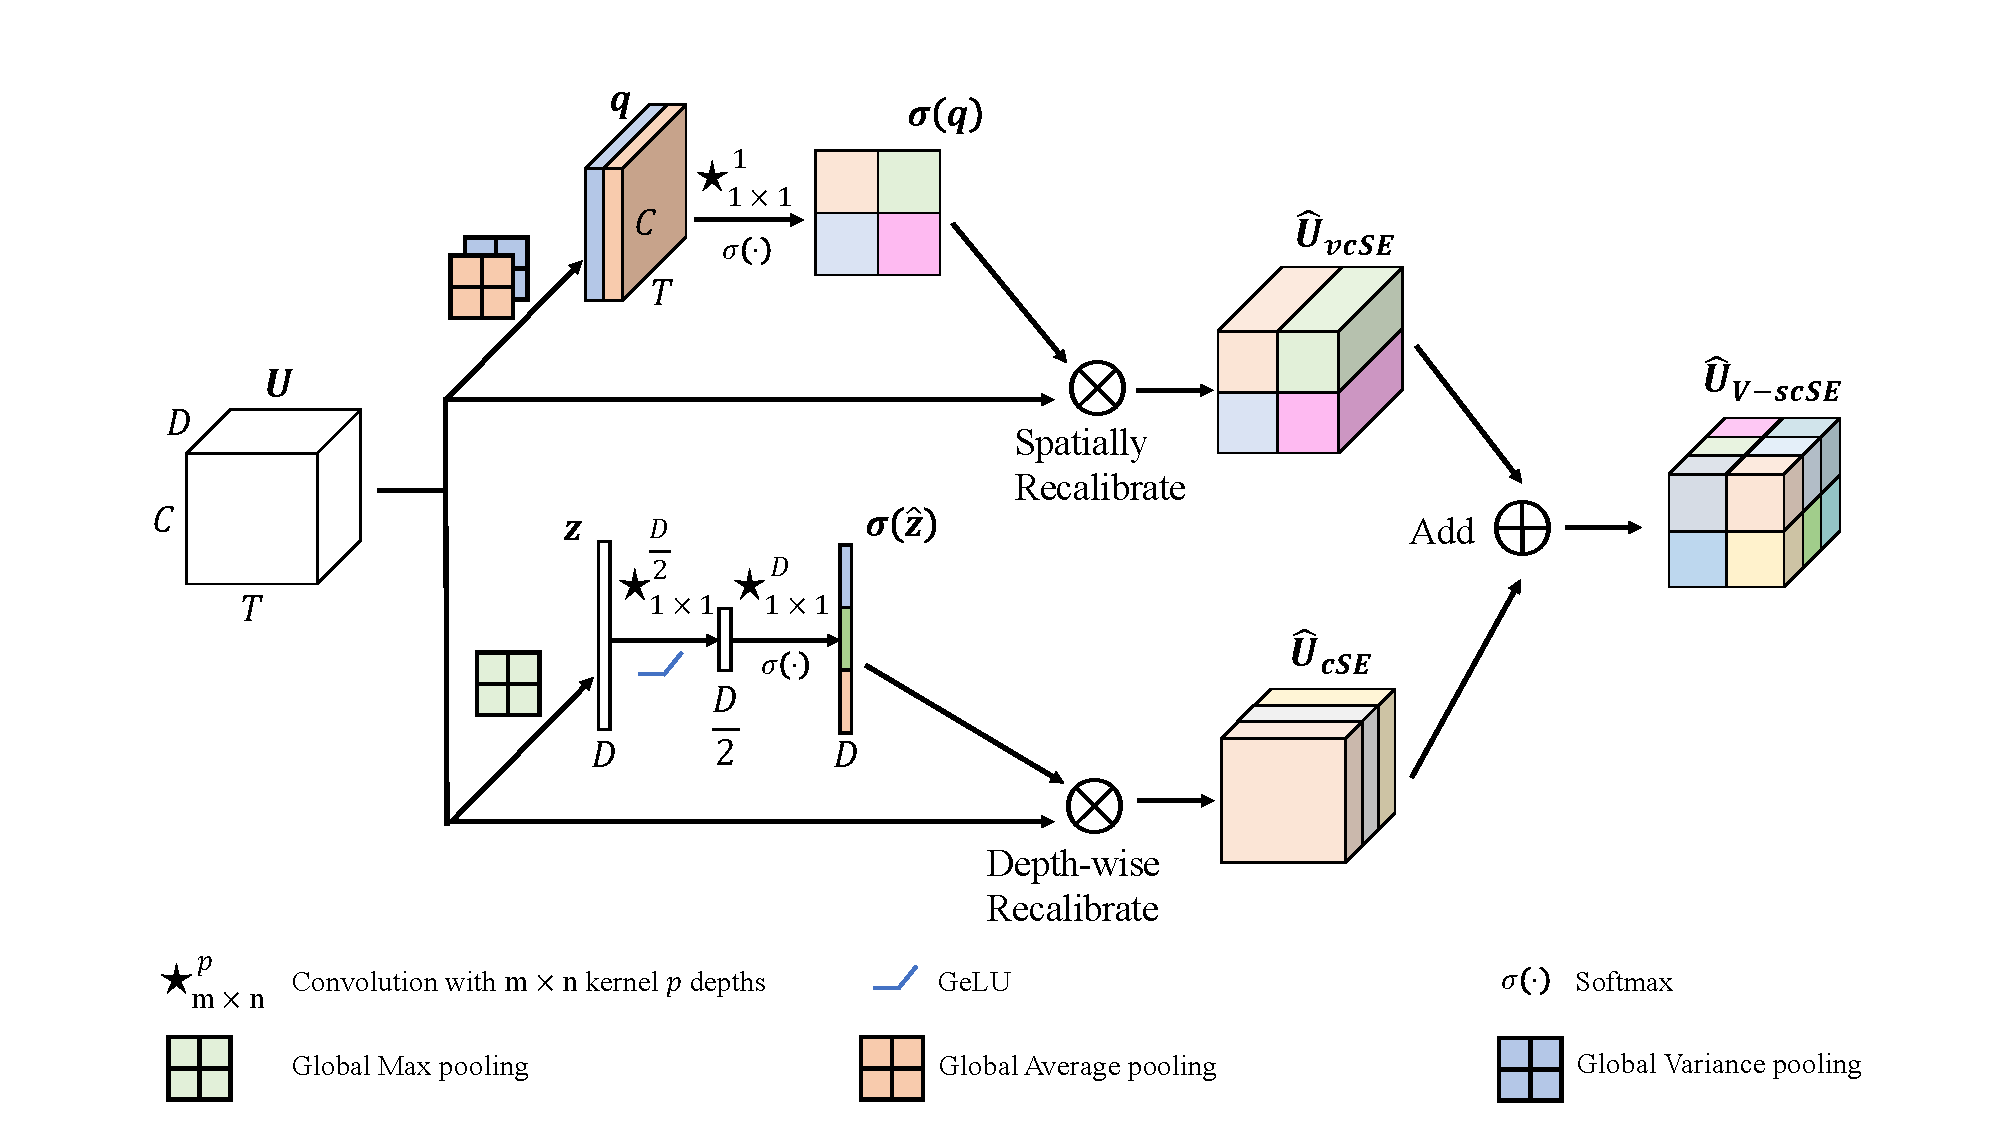
\includegraphics[width=\textwidth]{V-scSE.pdf}
  \caption{V-scSE结构}
  \label{fig:V-scSE}
\end{figure}

\section{基于密集连接改进的Inception模块}

尽管VSNet作为一款紧凑型端到端网络,能够在保持极小参数规模的前提下取得相对良好的性能表现,但其网络结构中仅采用单层卷积来进行时间特征和空间特征的提取,在一定程度上限制了模型对EEG信号中复杂时空信息的充分捕获和深入理解。因此,对VSNet进行进一步优化升级,以强化其提取EEG信号的高维时空特征的能力,是有一定意义的。需要说明的是,在后续的优化阶段,参数量仍然是论文设计网络时考虑的因素之一,但为了增强网络对高维时空特征的提取能力,将会引入更复杂的网络结构,导致参数量的不可避免的增长。因此,在后文中,参数量将不再如前一节中一般,作为衡量网络性能时的重点指标加以讨论。

\subsection{特征提取基础结构}

在VSNet中,特征提取的基础结构来自于ShallowConvNet中的单层卷积以及EEGNet中的深度可分离卷积,其中,提取空间特征的卷积层相较于提取时间特征的卷积层具有更少的卷积核,这是由于EEG信号的空间特征复杂度通常低于时间特征复杂度,时空信息具有不均衡性。例如,在BCI Competition IV Dataset 2B\cite{tangermann2012review}数据集中,仅仅使用了三个电极采集MI-EEG信号,使得空间信息相对时间信息更为稀疏。因此,在对VSNet的特征提取基础结构进行改进时,仍然沿用更关注时间特征的策略,即时间卷积层的复杂度要高于空间卷积层的复杂度,这一策略的目的在于使得模型具有捕捉高维时空特征能力的同时,防止模型因复杂度过高而在小样本数据集上过早地发生过拟合现象。

EEG原始输入具有时间和通道两个维度的信息,可以被视为具有空间信息的图像数据,因此,本节参考以下几种计算机视觉领域的经典模型,用于VSNet特征提取基础结构的改进:

1. Inception网络

Inception模块起源于经典的GoogLeNet模型\cite{szegedy2015going},并在计算机视觉图像分类任务中取得了优异的效果。传统卷积神经网络倾向于通过加深和拓宽网络结构以增进性能,然而这种做法伴随着参数数量的激增,不仅加大了计算负担,还可能导致过拟合问题。在这种背景下,Inception模块提出了多尺度特征并行抽取的策略,旨在保持网络稀疏性的同时,充分利用密集矩阵运算的高性能。典型的Inception-V1模块的结构如图~\ref{fig:Inception}~所示,其将不同大小的卷积层和最大池化层并行排列,并行地对输入数据执行多种卷积和池化运算,继而将提取到的不同尺度特征在深度维度上进行拼接。这种设计能够在单层网络内并行地提取输入数据在不同层次和粒度的特征信息,从而在高效扩展网络的深度和宽度的同时,有效削减参数规模,提升计算速度。此外,Inception模块中引入了1\times1卷积核,用以实现深度上的特征转化和降维,这种方式能够让模型学习到更为丰富的特征,同时降低计算成本。后续的论文中,Inception模块不断迭代优化,陆续引入了批归一化、深度可分离卷积、矩阵因子分解等技术,进一步提升了模型的性能\cite{szegedy2016rethinking}\cite{szegedy2017inception}。
\begin{figure}
  \centering
  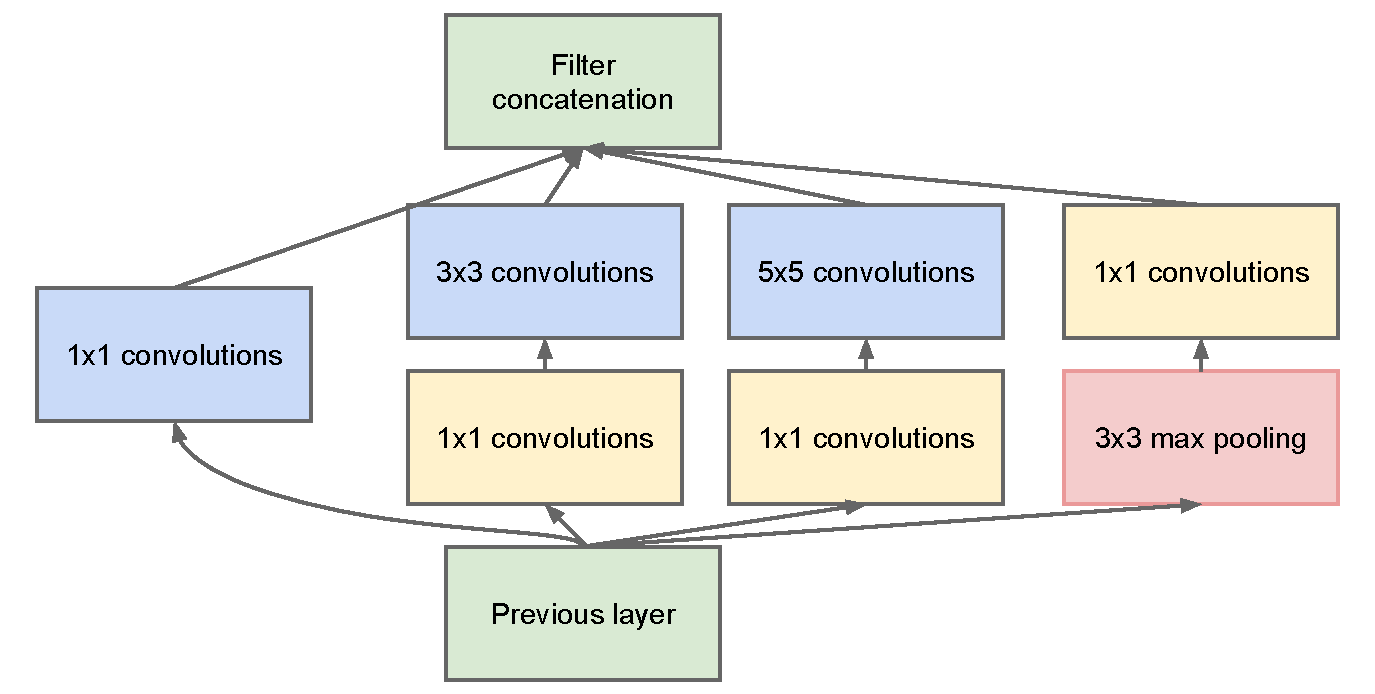
\includegraphics[width=\textwidth]{Inception.pdf}
  \caption{Inception结构}
  \label{fig:Inception}
\end{figure}

2. 残差神经网络

残差神经网络(Residual Network,ResNet)\cite{he2016deep}是计算机视觉图像识别领域的一个经典模型。ResNet研究发现了深度神经网络的退化现象(Degradation),即随着网络深度不断增加,模型准确率起初随深度上升,却在达到峰值后急剧下滑。针对这种现象,ResNet提出了残差学习框架,其核心思想是引入残差块(Residual Block),每个残差块通过快捷连接(Shortcut Connection)将输入信息直接输送至输出层,使得网络只需要专注学习输入与输出之间的残差信息,而非完整的映射关系。基础的ResNet由一系列残差块堆叠而成,残差块的结构如图~\ref{fig:ResNet}~所示。通过快捷连接,ResNet在训练过程中,梯度能够从深层网络直接回传至浅层,避免网络深度增加带来的训练困难和性能下降问题,从而提升深度神经网络的性能表现和训练效率。
\begin{figure}
  \centering
  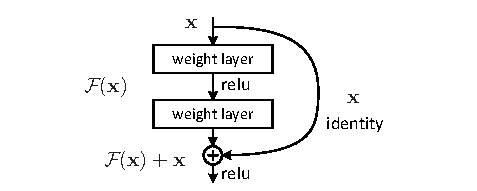
\includegraphics[width=\textwidth]{ResNet.pdf}
  \caption{残差块结构}
  \label{fig:ResNet}
\end{figure}

3. U-Net

U-Net模型\cite{ronneberger2015u}最初是为生物医学图像分割任务而设计,其具有优秀的性能,尤其在细胞、器官和病变区域的精确标注上表现出色,是医学图像分割领域的主流模型之一。U-Net的独特之处在于其采用了对称的编码-解码结构(Encoder-Decoder)和跳跃连接(skip connection),其结构如图~\ref{fig:UNet}~所示。编码器通过连续的卷积和下采样层对输入图像进行深度特征提取和空间压缩,提炼出高级抽象特征;解码器部分则通过上采样和卷积恢复到与输入图像相同的空间分辨率,同时保留详细的定位信息。跳跃连接将编码器各阶段的特征图直接传递给相应的解码器阶段,有效地结合了包含更多细节信息的浅层特征和包含更多高级语义信息的深层特征,从而在图像分割任务中能够取得更为精细的分割效果。同时,U-Net模型结构简单,易于训练,能够缓解小样本数据集上的过拟合问题。
\begin{figure}
  \centering
  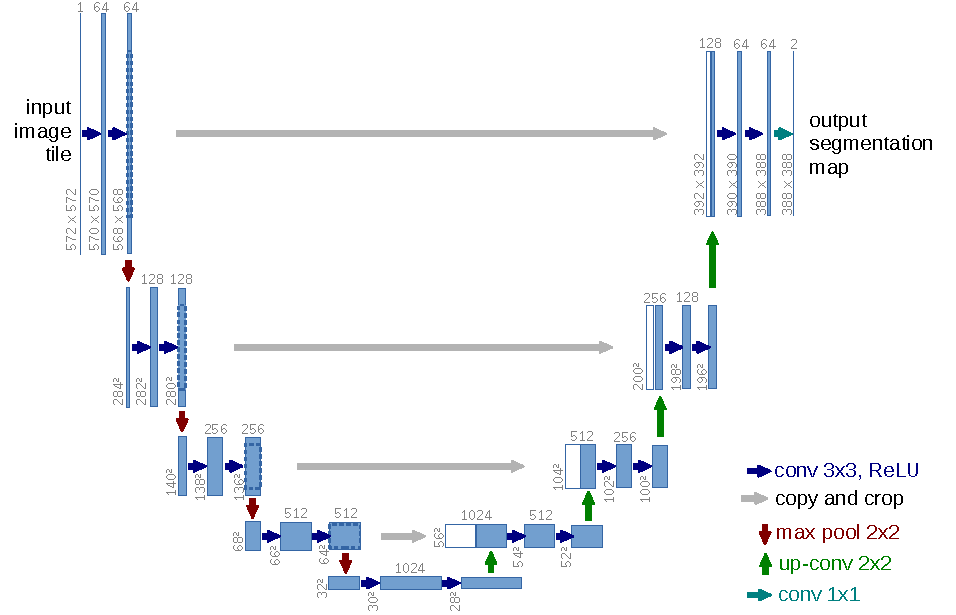
\includegraphics[width=\textwidth]{UNet.pdf}
  \caption{U-Net结构}
  \label{fig:UNet}
\end{figure}

在这三种模型中,Inception和ResNet均在图像分类任务中展现出了优秀的性能。Inception通过同一层网络内的多尺度特征并行抽取,在不显著增加网络深度的前提下,实现了特征提取的广度与效率的提升。ResNet通过引入快捷连接,解决了深度神经网络训练过程中的梯度消失和退化问题,增强了深层次网络的训练效率和性能表现。U-Net则在生物医学图像分割领域取得了优秀的表现,医学图像的语义信息较为简单,且结构较为固定,因此高级语义信息和低级特征都相对重要,U-Net通过跳跃连接保留并融合了这两类信息,同时,U-Net参数量较小,不容易在小样本数据集上发生过拟合现象。论文选择将U-Net迁移至MI-EEG分类任务中,是因为EEG信号具有与生物医学图像类似的生理特性,如特征相对简单、数据集规模偏小等。

为了验证Inception、ResNet与U-Net在EEG信号分类任务中的性能,论文在BCI Competition IV Dataset 2A数据集上进行实验对比。在实验设置中,统一将三种模型的网络深度调整为三层,并对其他关键参数如卷积核大小、学习率等进行了固定,此外,对这三种模型的原始代码进行了调整,使得其适应MI-EEG分类任务。实验结果如表~\ref{tab:Incep-Res-U}~所示,主要展示准确率(Accuracy,ACC)和Kappa一致性系数(Kappa)指标,这两项指标是数据集中九位受试者的平均表现。
\begin{table}[ht]
  \centering
  \caption{Inception、ResNet、U-Net实验结果对比}
  \label{tab:Incep-Res-U}
  \begin{tabularx}{\textwidth}{CCC}
    \toprule
    Models & ACC(\%) & Kappa \\
    \midrule
    Inception & \textbf{67.40} & \textbf{0.56} \\
    ResNet & 56.94 & 0.43 \\
    U-Net & 62.27 & 0.50 \\
    \bottomrule
  \end{tabularx}
\end{table}

实验数据显示,Inception模型在这三种模型中具有最优的性能表现,U-Net次之,ResNet的表现则相对较差。这可能是因为同样的网络深度下,Inception模型得益于多尺度并行特征提取机制,能更全面地捕获EEG信号的多种特征。相比之下,U-Net虽然通过跳跃连接有效地结合了EEG信号的低层特征和高层语义信息,但在解码器阶段,U-Net将特征图重建至原始空间尺寸的过程可能为分类任务引入了不必要的复杂性。ResNet的快捷连接在较浅层网络结构中可能未能完全发挥其优势,更适用于深层次网络。实验结果与过往研究中关于浅层网络更适合MI-EEG分类任务的研究结论相互印证。综上所述,论文选用Inception模块用于VSNet特征提取结构的改进,旨在保持模型简洁高效的同时,在MI-EEG分类任务中取得更好的性能。

\subsection{密集连接}

在前一节中,论文选取了Inception模块作为改进VSNet的方案,然而,值得注意的是,U-Net在处理MI-EEG分类任务时同样展现了一定的优势。由于EEG信号的特征相对简单,因此低级特征与高级语义信息都相对重要,U-Net因其特殊的跳跃连接结构有效地融合了这两种信息,然而,U-Net中通过解码器阶段将特征图恢复至原始空间尺寸的操作并非必要,因为在分类任务中,这种重建过程可能导致额外的计算负担且对分类性能的提升效果不明显。因此,在对VSNet进行改进时,论文从U-Net兼顾低级特征与高级语义信息的策略中得到启发,同时对不必要的特征图空间尺寸还原过程进行规避,以构建一个既能充分利用EEG信号中各级别特征信息,又具备高效计算能力的改进模型。

Gao Huang等人于2016年提出了密集连接网络\cite{huang2017densely}(Dense Convolutional Network,DenseNet)。在ResNet的基础上,DenseNet提出了一种更为激进的连接模式:引入从任意层到后续层的直接连接,即密集连接(Dense Connection)。DenseNet的第 \(l\) 层接收所有前序特征图为输入,其输出为 \(x_l\):
\begin{equation}
  x_l = H_l([x_0, x_1, ···, x_{l-1}])
  \label{eq:dense-conn}
\end{equation}
其中,\([x_0, x_1, ···, x_{l-1}]\) 代表第 \(0, ···, l-1\) 层的输出特征图,\(H_l(·)\) 代表非线性转换复合函数,可能包括一系列的批量归一化、ReLU、池化及卷积操作。密集连接的结构如图~\ref{fig:denseBlock}~所示。
\begin{figure}
  \centering
  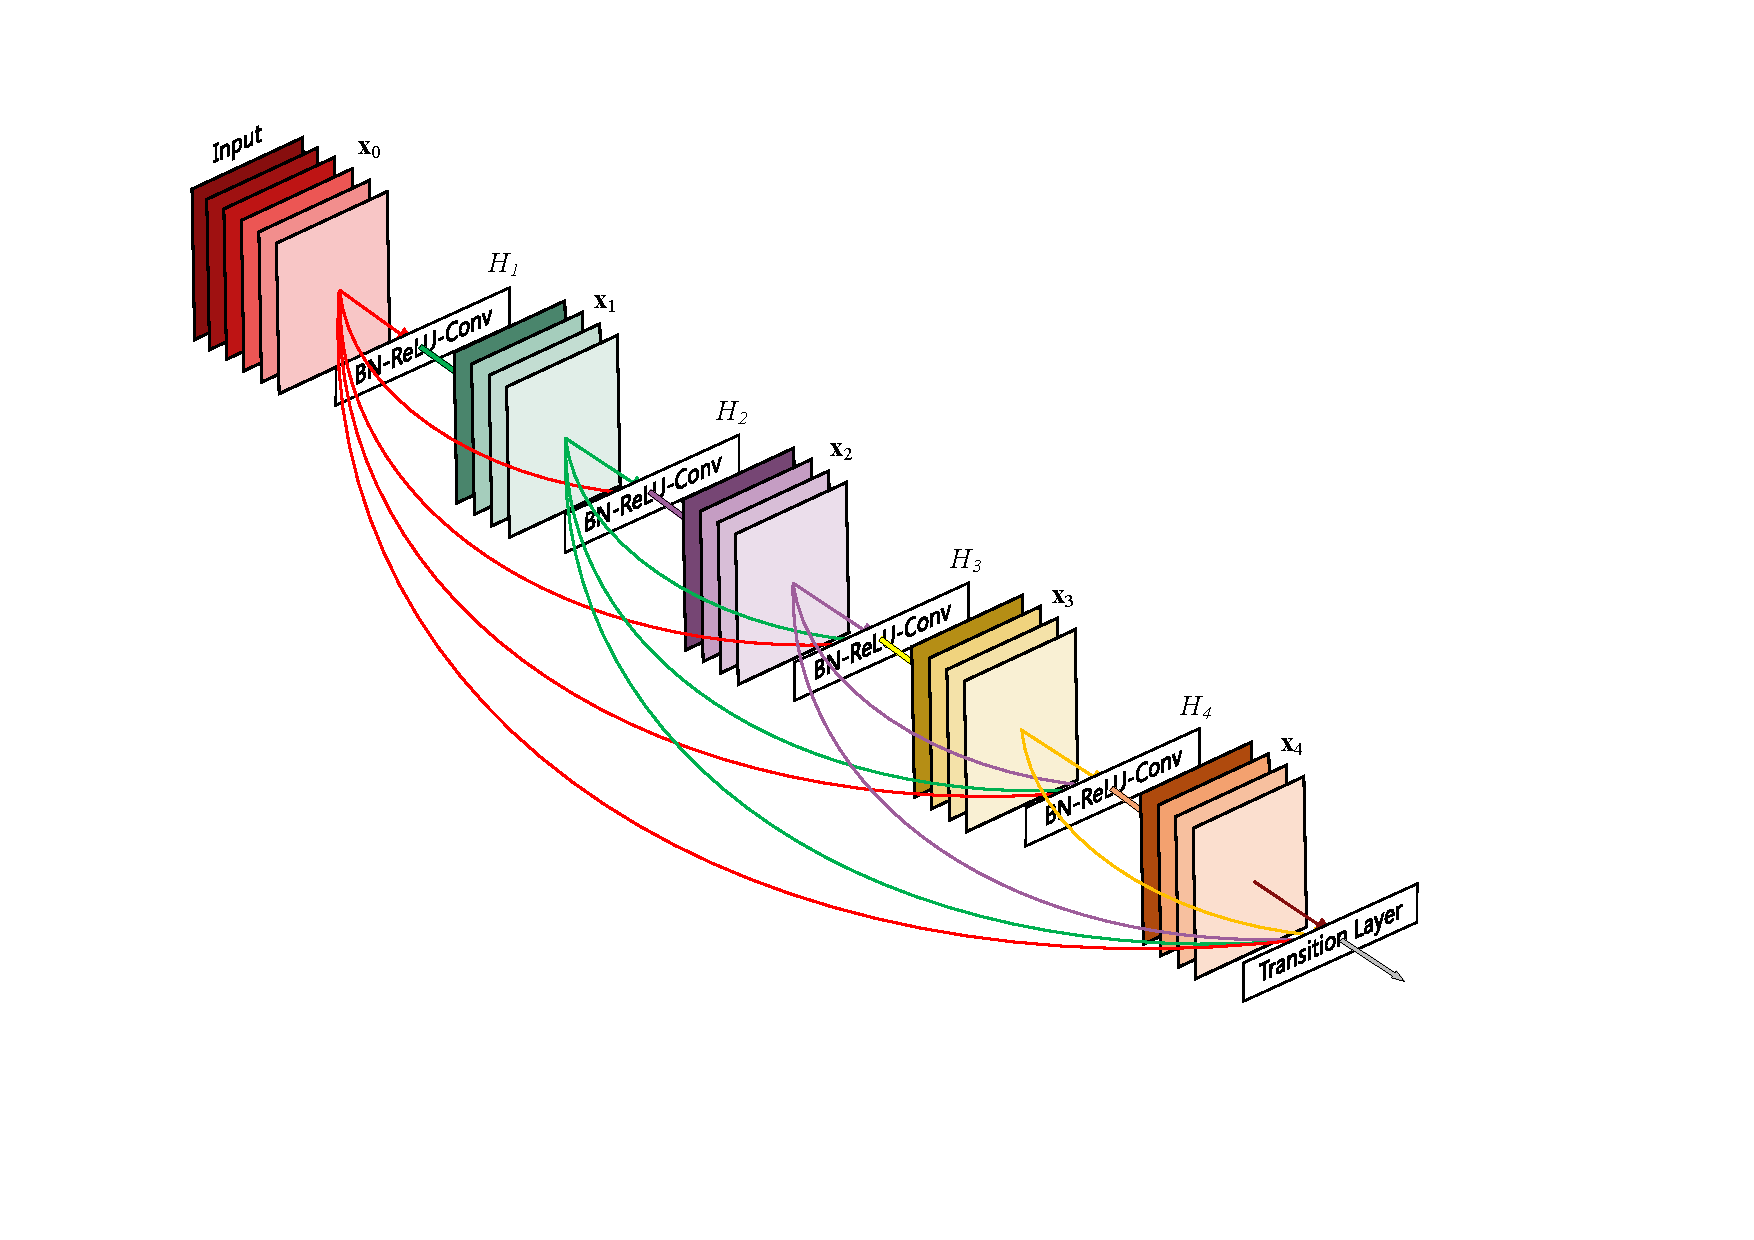
\includegraphics[width=0.8\textwidth]{denseBlock.pdf}
  \caption{密集连接结构}
  \label{fig:denseBlock}
\end{figure}

在密集连接模块中,所有的前序特征图通过Concentrate在深度维度上连接在一起,因此,在一个密集连接模块中所有特征图的大小是相同的。DenseNet提出了Transaction模块用于连接两个相邻的密集连接模块,并通过池化操作对特征图进行下采样,从而减小特征图的大小。

通过密集连接的方式,网络中的每一层都能够访问并整合所有前序层提取出的特征信息,进而充分利用EEG信号中的低层特征细节和高层语义信息。相较于U-Net中的编码-解码结构,密集连接无需经历数据空间的重建过程,即可实现特征的有效复用。此外,DenseNet中的Transition模块也为实现特征图的下采样提供了思路。

\subsection{基于密集连接改进的Inception模块}

原始的Inception模块和密集连接模块在计算机视觉图像分类任务中都取得了优秀的表现,在设计上,它们都考虑到了图像数据在空间维度具有等价的重要性。然而,EEG信号的时空信息具有不均衡的重要性,通常情况下,时间维度往往比空间维度蕴含更为丰富的信息。与此同时,研究指出\cite{lawhern2018eegnet},当设计用于提取EEG特征的卷积核时,将时间卷积核长度设置为EEG信号采样率的一半,可以有效地捕获2Hz及以上频段的信号信息。因此,在处理EEG信号时,时间卷积核的长度应当依据EEG信号的实际采样率来灵活设定,以便提取不同频率成分的信号特征。

鉴于上述EEG信号与图像数据的特性差异,原始的Inception模块和密集连接模块在未经适当改造的情况下,并不适合直接应用于MI-EEG分类任务。为此,有必要对这些模块进行针对性的调整和优化,以适应EEG信号的特性和MI-EEG分类任务的需求。

鉴于EEG信号的时间维度蕴含着更为丰富的信息,论文对VSNet中的时间卷积层进行进一步的优化。论文将Inception模块中的卷积核概念转化为针对时间序列的一维卷积(尽管在实现时仍采用二维卷积),舍弃了原始Inception模块中针对图像数据的空间可分离卷积设计。为了更好地匹配EEG信号的采样特性及其内在频率成分,依据EEG信号的采样频率 \(sfreq\) 来动态调整Inception模块各个分支的时间卷积核大小,具体公式如下:
\begin{equation}
  kernel_i = sfreq \times time\_unit_i, \quad time\_unit_i \in \{0.1, 0.3, ···, 0.9\}
  \label{eq:kernel_cal}
\end{equation}
其中,\(kernel_i\) 表示Inception模块第 \(i\) 个分支所使用的卷积核大小,而 \(sfreq\) 是EEG信号的采样频率,\(time\_unit_i\)  则为卷积核对应的时间单位,其取值范围分布在0.1秒至0.9秒的奇数间隔内。这样设置卷积核大小是为了更全面地捕捉EEG信号中不同频率成分的特征信息,同时避免因卷积核大小过于接近而导致提取的特征之间重叠度过高。例如,当采样周期设定为0.5秒时,卷积核大小将是采样率的一半,进而能够有效地捕获到2Hz及更高频段的EEG信号特征。


原始Inception模块中采用了瓶颈层进行特征降维,然而考虑到在VSNet架构中,时间卷积层前置了瓶颈层对EEG信号进行适当的特征升维以挖掘更多信息,论文决定舍弃原始Inception模块中可能导致EEG信号特征损失的降维瓶颈层设计方案。

在构建VSNet时,空间卷积层有两种不同的方式融入基于Inception改进的时间卷积层之后,一种是在每个Inception模块内部的分支结构上增加空间卷积层,另一种则是在整个Inception模块之后附加空间卷积层。图~\ref{fig:ts-incep}~展示了这两种引入方式的区别,将这两种方式分别称为分支内融合(Inception-In)和模块后融合(Inception-After),需要说明的是,图中省略了网络的其他结构,如瓶颈层等,以尽可能简洁地展现不同引入方式的差异。
\begin{figure}
  \centering
  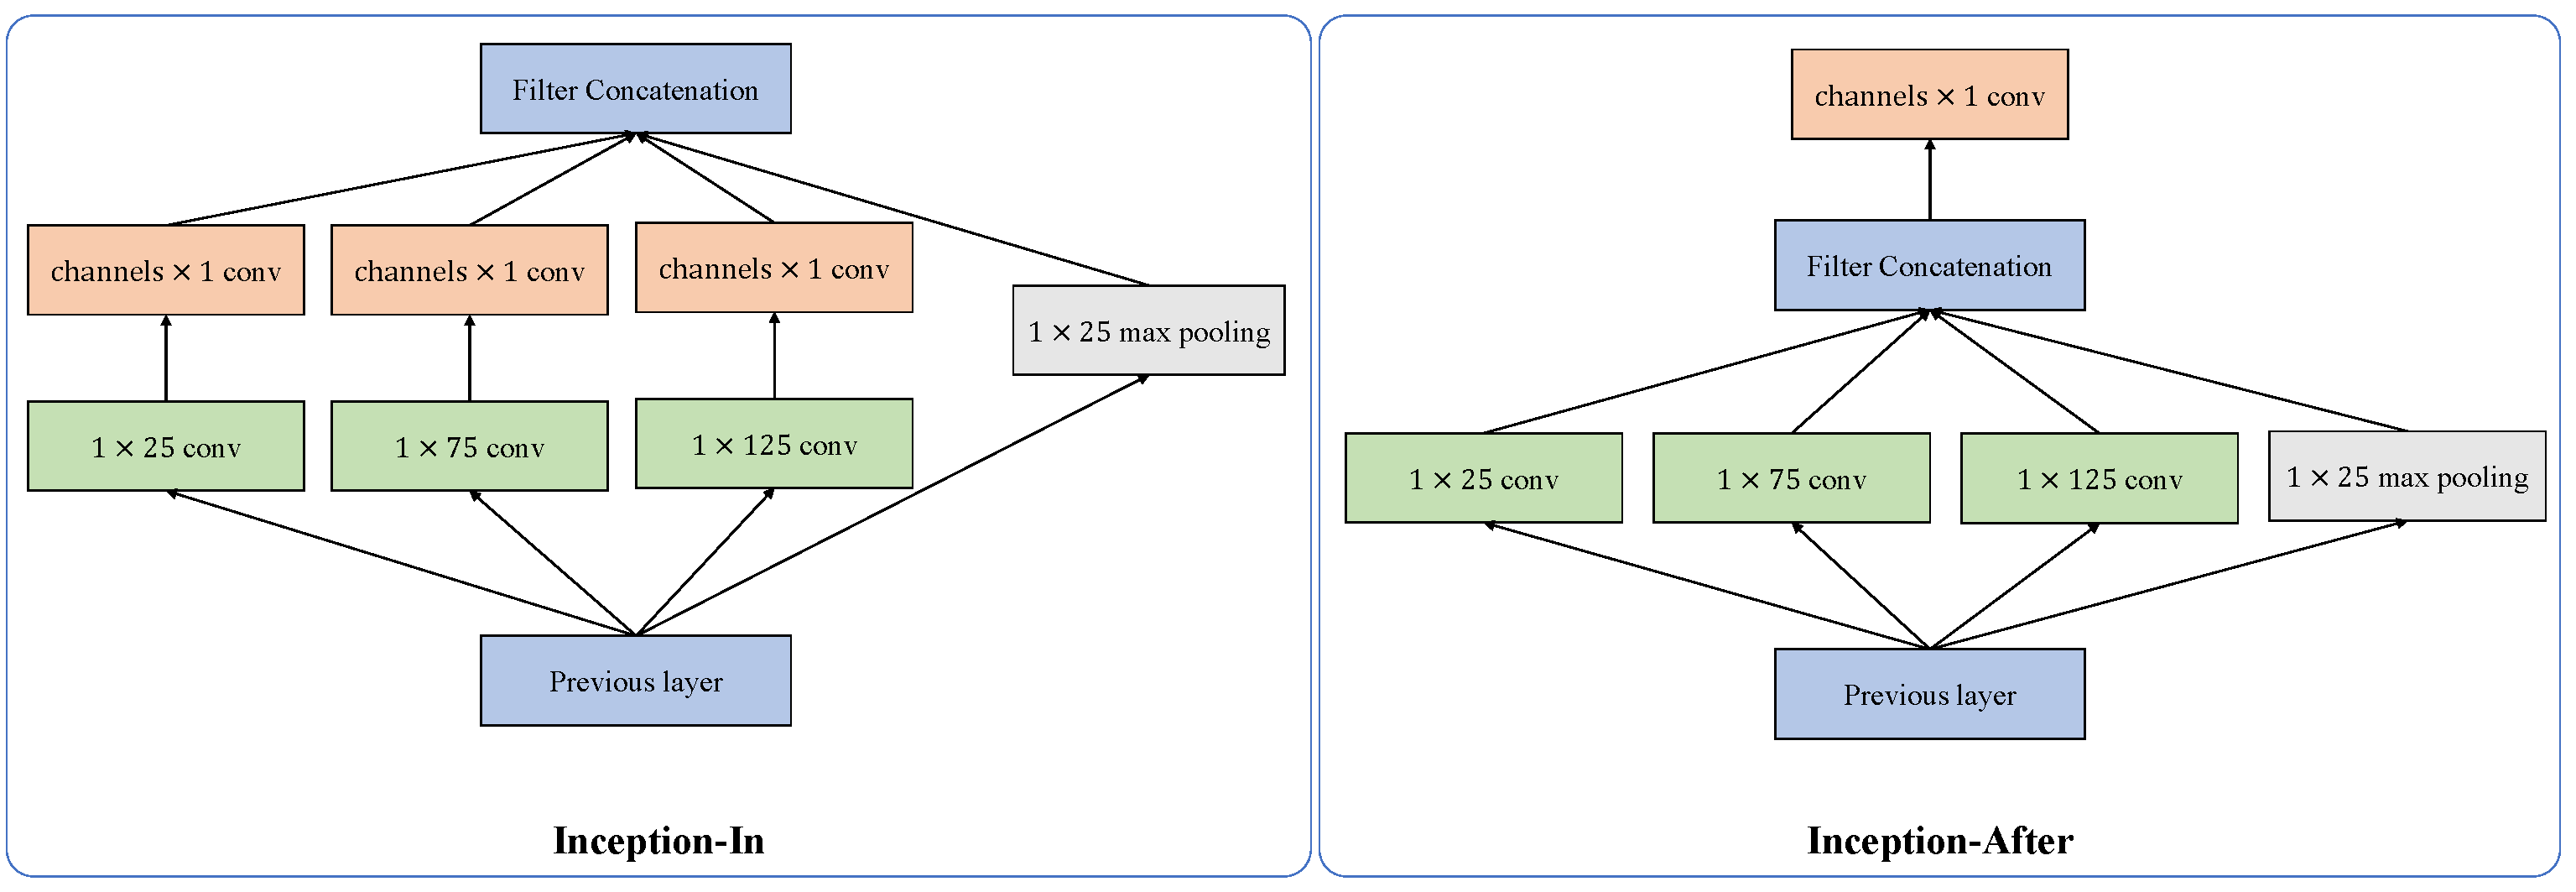
\includegraphics[width=\textwidth]{ts-incepv2.pdf}
  \caption{Inception模块引入空间卷积层的方式}
  \label{fig:ts-incep}
\end{figure}

为了比较Inception-In与Inception-After的性能差异,论文在BCI Competition IV Dataset 2A数据集上设计实验进行对比。在实验设置阶段,固定了Inception模块的层次数量、分支数量等参数,实验结果如表~\ref{tab:ts-inception}~所示。在此,重点关注两项评价指标——准确率(Accuracy, ACC)和Kappa一致性系数(Kappa),这两项指标均基于数据集中九位受试者的平均表现。实验结果显示,Inception-After方式在准确率和一致性系数上均表现更优。这一优势可能源自两方面的原因:一方面,虽然Inception-In模式借鉴了FBCSP算法的分频段处理思路,但在Inception分支内部直接进行空间特征提取的过程中,损失了部分空间全局信息;另一方面,Inception-In结构具有相对更大的参数规模,这可能导致模型在有限样本条件下更容易出现过拟合现象。基于以上分析和实验验证,论文选择以Inception-After的方式布局时间卷积层与空间卷积层。
\begin{table}[ht]
  \centering
  \caption{Inception-In、Inception-After实验结果对比}
  \label{tab:ts-inception}
  \begin{tabularx}{\textwidth}{CCC}
    \toprule
    Models & ACC(\%) & Kappa \\
    \midrule
    Inception-In & 63.31 & 0.51 \\
    Inception-After & \textbf{75.35} & \textbf{0.70} \\
    \bottomrule
  \end{tabularx}
\end{table}

在以上改进的基础上,为了同时充分挖掘和利用EEG信号中的低级特征与高级语义信息,论文选择在Inception模块中引入密集连接的概念,替代原有的时间卷积核设计。在DenseNet中,有两种不同构造的密集连接模块,分别是基础密集连接模块(Basic Dense Block)和带有瓶颈层的密集连接模块(Bottleneck Dense Block),它们的区别主要体现在非线性转换复合函数 \(H(·)\) 的设计上:

1. 基础密集连接模块(Basic Dense Block):

其非线性转换复合函数定义为: \(H(·) = BN + ReLU + 3 \times 3\;conv\)。

2. 瓶颈密集连接模块(Bottleneck Dense Block):

其非线性转换复合函数更为复杂,包括两个卷积层、两次BN和ReLU激活:\(H(·) = BN + ReLU + 1\times1\;conv + BN + ReLU + 3 \times 3\;conv\)。加入瓶颈层的主要原因在于降低特征维度的数量,从而提升模型计算效率。

论文对Inception模块第 \(i\) 个分支采用了基于Bottleneck Dense Block的密集连接模块,并对其进行了适当调整,定义的非线性转换复合函数 \(H(·)\) 如下:
\begin{equation}\label{eq:dense-kernel}
  \begin{split}
    &H(·) = BN + GeLU + 1\times1\;conv + BN +  1 \times kernel_i\;conv + Dropout \\
    &kernel_i = sfreq \times time\_unit_i, \quad time\_unit_i \in \{0.1, 0.3, ···, 0.9\}
  \end{split}
\end{equation}
相较于原始的Bottleneck Dense Block,论文在前文研究的基础上做出了以下改进,分别为:根据EEG信号的特性调整了卷积核大小;选用性能更优的激活函数GeLU替代ReLU;引入了Dropout层,以进一步缓解过拟合现象。

经过上述基于密集连接策略的改进,新构建模型的结构如图~\ref{fig:incep-dense}~所示,将其命名为DI-VSNet。Dense-Inception module构成了时间卷积层,其内部的各个分支均由一系列改进版的Bottleneck Dense Block紧密堆叠而成,形成密集连接结构,用以同时获取浅层和深层的时间特征。每个分支提取的特征图在深度维度上进行聚合,并通过Transaction模块进行深度压缩和特征整合,以进一步提升模型的表达能力和计算效率。需要说明的是,Dense-Inception module的数量,以及Dense-Inception module的分支数量、Dense block的数量,都是可调的超参数。
\begin{figure}
  \centering
  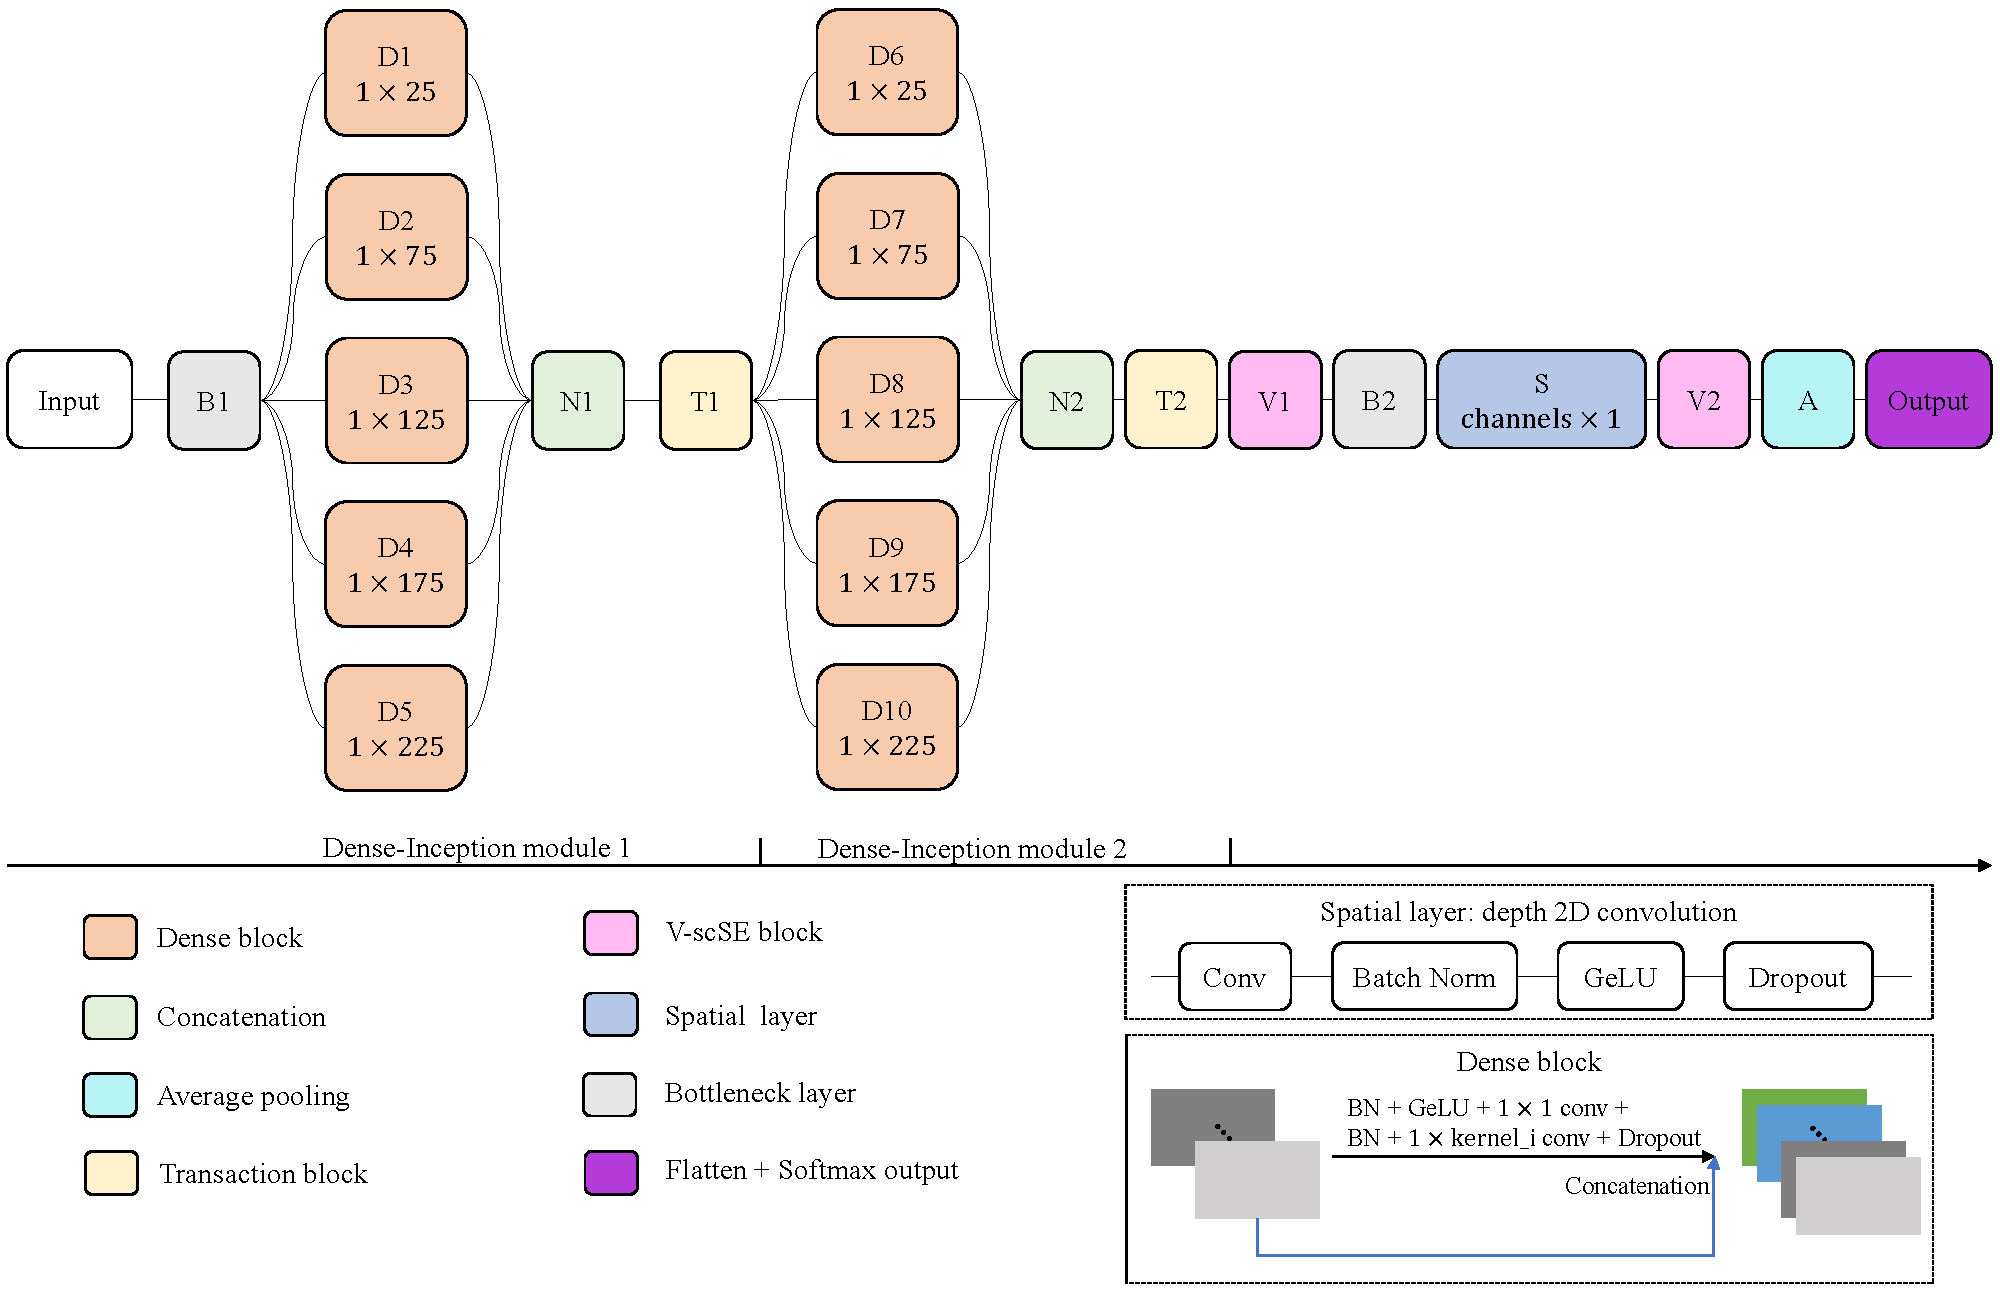
\includegraphics[width=\textwidth]{incep-dense.pdf}
  \caption{DI-VSNet结构}
  \label{fig:incep-dense}
\end{figure}

\section{基于软阈值化改进的Transformer模块}

卷积神经网络中,尽管卷积层因其局部感受野能够出色地捕获信号中的局部时空特征,但对于那些跨越较长时间跨度和空间分布的复杂交互信息,其建模能力受限。而Transformer模型因其自注意力机制(Self-Attention)可以在不考虑输入位置顺序的情况下,灵活地捕捉并编码任意两点之间的相互依赖关系,从而能够更有效地理解和处理长距离依赖,但与此同时,其可能无法充分提取局部时空特征。银日,论文选择将两者进行结合,用于MI-EEG分类任务。

原始的Transformer模型是编码器-解码器(Encoder-Decoder)结构,编码器负责对输入序列进行编码,提取其蕴含的语义和上下文信息,解码器负责基于编码器提供的上下文信息生成目标序列,即编码器用于对输入序列的变换加权,解码器用于生成目标序列。在MI-EEG分类任务中,Transformer模型只用来提取长距离依赖信息,而无需生成目标序列,因此,只需要使用编码器。

\subsection{Transformer并行连接的模型}

\subsection{Transformer编码器构建}

\subsection{基于软阈值化改进的Transformer}


\section{基于Inception和混合注意力的运动想象脑电图分类网络HIT-Net}


\section{本章小结}